\documentclass[sigchi, screen, nonacm]{acmart}

\setlanguage{\german}

% --- Own includes -------------------------------------------------------------
\providecommand{\tightlist}{%
  \setlength{\itemsep}{0pt}\setlength{\parskip}{0pt}}

% make images fit into the page
\usepackage{graphicx}
\makeatletter
\def\ScaleWidthIfNeeded{%
 \ifdim\Gin@nat@width>\linewidth
    \linewidth
  \else
    \Gin@nat@width
  \fi
}
\def\ScaleHeightIfNeeded{%
  \ifdim\Gin@nat@height>0.9\textheight
    0.9\textheight
  \else
    \Gin@nat@width
  \fi
}
\makeatother
\setkeys{Gin}{width=\ScaleWidthIfNeeded,height=\ScaleHeightIfNeeded,keepaspectratio}%

% new line after subheading
\makeatletter
\def\subsubsection{\@startsection{subsubsection}{3}%
  \z@{.5\linespacing\@plus.7\linespacing}{.5\linespacing}%
  {\normalfont\itshape}}
\makeatother

\usepackage{longtable}

% --- Begin of Document --------------------------------------------------------

\begin{document}

\title{Dokumentation zur App "Grüni"}

% Autoren

\author{Robert Ackermann}
\affiliation{\institution{Fachhochschule Erfurt}}
\email{robert.ackermann@fh-erfurt.de}

\author{Hannes Dröse}
\affiliation{\institution{Fachhochschule Erfurt}}
\email{hannes.droese@fh-erfurt.de}

\author{Dennis Krischal}
\affiliation{\institution{Fachhochschule Erfurt}}
\email{dennis.krischal@fh-erfurt.de}

\author{Livia Schumm}
\affiliation{\institution{Fachhochschule Erfurt}}
\email{livia.schumm@fh-erfurt.de}

% Abstract

\begin{abstract}
Im Folgenden behandeln wir Anfänge, Entwicklung und Ergebnisse des Semester-Projektes "Grüni" im Rahmen des Medienprojekt-Moduls. Grüni ist die Vision einer Anwendung um Nutzern das Gärtnern sowie das gärtnern lernen zu erleichtern.
\end{abstract}

% Keywords
\keywords{gärtnern, lernen, AR, Vision, Zukunft, Pflanzen, Technik}

% parse and render metadata
\maketitle

% Einfügen des Beitrag-Textes
\hypertarget{die-idee}{%
\section{Die Idee}\label{die-idee}}

Die Idee einer Gärtnerhilfe-Anwendung entstand bereits Anfang April 2020
während des ersten Brainstormings. Im ersten Treffen des Moduls, am
20.04.2020 fanden wir vier - Robert Ackermann, Hannes Dröse, Dennis
Krischal und Livia Schumm - uns in einer Projektgruppe zusammen und
führten am selben Tag unser erstes Webex-Meeting durch, in dem über
verschiedene Ideen beratschlagt wurde. Für die Aufgabenstellung mit dem
Motto ``Future Interfaces'' sollten zwei Teilprojekte abgedeckt werden:

\begin{enumerate}
\def\labelenumi{\arabic{enumi}.}
\tightlist
\item
  Die Entwicklung einer \protect\hyperlink{vision}{Vision}, also die
  Konzeption einer zukunftsweisenden intuitiven Interaktion mit
  digitalen Inhalten und deren Darstellung in Form eines Visionsvideos
\item
  Die Entwicklung eines \protect\hyperlink{prototyp}{Prototyps} dieser
  Vision, sprich die Ausarbeitung einer interaktiven Anwendung
\end{enumerate}

Unsere Projektidee sollte also sowohl innovativ als auch in Teilaspekten
umsetzbar sein, jedoch sollten wir uns vorerst mehr auf die Vision als
auf den Prototypen konzentrieren. Es entstand eine Auswahl folgender
Projektthemen:

\begin{itemize}
\tightlist
\item
  Gardening - App zum Gärtnern lernen, unterstützt und lehrt das
  Gärtnern
\item
  Kontaktloses Bezahlen und papierlose Kassenbons
\item
  Verwaltung - Online Identitätsfeststellungen, Digitale Formulare
\item
  Antlitzdiagnostik - Apps analysieren den Gesundheitszustand,
  appgestützte Ferndiagnose mit Ärzten
\end{itemize}

Der gemeinsame Favorit zeichnete sich im Gespräch jedoch schnell ab und
nach einer kurzen Themenabstimmung mit den betreuenden Dozenten stand
die Richtung in den Gardening-Bereich also fest.

\hypertarget{recherche}{%
\subsection{Recherche}\label{recherche}}

Der nächste Schritt, nachdem eine Projektrichtung festgesteckt wurde,
ist die Recherche in diesem Bereich. Im Fall des Gardenings stellen sich
vor allem drei Fragenfelder:

\begin{enumerate}
\def\labelenumi{\arabic{enumi}.}
\tightlist
\item
  Wie sieht Gärtnern aktuell überhaupt aus, woran besteht Bedarf und in
  welche Richtung gehen die Trends der Zukunft?
\item
  Welche Apps, Anwendungen und Projekte gibt es bereits und welche sind
  in der Entwicklung?
\item
  Wie sehen die technischen Möglichkeiten aus? Welche Sensoren,
  Messtechniken o.ä. werden in der Landwirtschaft gebraucht oder sind im
  Garten einsetzbar?
\end{enumerate}

\textbf{Anmerkung:} Im Folgenden werden nur einige, wesentliche Aspekte
dieser Recherche zusammengetragen, weitere gesammelte Informationen und
Artikel finden sich in unserem Projekt unter den Recherchen im
Managment-Tool Asana\footnote{Allgemeine Recherche und Trends:
  https://app.asana.com/0/1172859492234369/1172897938417709\\
  Pflanzen Apps:
  https://app.asana.com/0/1172859492234369/1172897938417707\\
  Sensoren und Messtechnik:
  https://app.asana.com/0/1172859492234369/1172859492239381}.

\hypertarget{trends-und-aktuelle-entwicklung-des-guxe4rtnerns}{%
\subsubsection{Trends und aktuelle Entwicklung des
Gärtnerns}\label{trends-und-aktuelle-entwicklung-des-guxe4rtnerns}}

Dass die Beliebtheit von Gärten, Pflanzen und Natur steigt, merkt schon
alleine wer sich im eigenen Umfeld umsieht. Zahlreiche Artikel, Blog-
und Social Media-Beiträge zeigen die Trends des \textbf{Urban
Gardening}, des \textbf{Urban Jungles}, des \textbf{DIY} (Do It
Yourself) auf.

Laut dem Zukunftsinstitut\footnote{Artikel ``Die Zukunft ist ein
  Garten'' -
  https://www.zukunftsinstitut.de/artikel/wohnen/die-zukunft-ist-ein-garten/}
ist die Zahl der Menschen mit Garten oder Balkon in Deutschland zwischen
2007 und 2011 von 50 Millionen auf 55 Millionen gestiegen, ebenso sinkt
das Durchschnittsalter von Kleingarten-Pächtern stetig ab\footnote{Artikel
  vom 22.11.2017: ``Blick in die Zukunft: So leben wir im Garten 2030''
  -
  https://taspo.de/kategorien/blick-in-die-zukunft-so-leben-wir-im-garten-2030/}.
Der Trend geht hin zur Begrünung von Gärten, Balkonen, Terrassen, zur
Gründung sowie Nutzung von Gemeinschafts- und Nachbarschaftsgärten, vor
allem bei der naturhungrigen Stadtbevölkerung und die Gartenbranche
stellt sich langsam auf eine \textbf{neue, jüngere Zielgruppe} ein. Die
steigende Beliebtheit des Gärtnerns jeglicher Art liegt unter anderem im
Ausgleich, das es zum stressigen Stadtalltag bieten kann, aber auch in
seiner guten Vereinbarkeit mit dem Nachhaltigkeits-Trend. Verschiedene
Faktoren lassen haufenweise individuelle und clevere Ansätze entstehen.
Die Nachfrage nach Bio-Produkten und Nutzpflanzen und dafür möglichst
einfachen aber möglichst autonomen Systemen ist groß.

Der Platzmangel in Städten verlangt z.B. nach vertikalen Lösungen:

\begin{itemize}
\tightlist
\item
  ``Pflanzetageren'': Versetzt angeordnete, kleeblattförmige Gefäße, die
  sich hoch stapeln lassen\\
\item
  ``Minigarden'': vertikales Pflanzsystem, Begrünung von Wänden oder
  kompletter Balkonbrüstung\\
\item
  ``Skyplanter'': Pflanzen wachsen in einer Art umgedrehtem Blumentopf
  von der Decke herab nach unten
\end{itemize}

Doch nicht nur das Interesse in Richtung zurück zum Ursprünglichen, zur
Natur ist groß, sondern auch innovative, konnektive Lösungen sind
gefragt, die das Leben in Haus und Garten durch \textbf{smarte Technik}
vereinfachen. In seinem Vortrag auf dem DIY Garden Summit 2017 in
Berlin\footnote{Artikel vom 22.11.2017: ``Blick in die Zukunft: So leben
  wir im Garten 2030'' -
  https://taspo.de/kategorien/blick-in-die-zukunft-so-leben-wir-im-garten-2030/}
erklärte Christian May, Geschäftsführer von Kärcher, wie ein Tag im
Garten des Jahres 2030 aussehen könnte:

\begin{quote}
Während eines gemütlichen Frühstücks in der Sonne auf meiner Terrasse
fällt mein Blick auf den Grill: Ihn umgeben unschöne Überbleibsel vom
gestrigen Grillfest. Doch dem Hochdruckreiniger fehlt der spezielle
Aufsatz für Rußflecken. Schnell ist die passende Vorlage gefunden und
kurz darauf druckt der 3D-Drucker den fehlenden Aufsatz aus und die
Arbeit kann beginnen. Da ich nun schon einmal im Garten bin, kümmere ich
mich auch gleich um meine Blumenbeete. Während ich mich umschaue, zeigen
mir einzelne Pflanzen auf meiner Smart-Brille an, dass sie nicht genug
Sonne bekommen und umgepflanzt werden müssen. Am Nachmittag ist es Zeit
für meinen Videokurs zum Thema Pflanzen, Pflegen und Ernten seltener
Gemüsesorten -- meinem Steckenpferd. Meine Expertise auf dem Gebiet
teile ich gerne und inzwischen lauschen meinen interaktiven
wöchentlichen Livestreams interessierte Hobbygärtner und Landwirte aus
Kanada, Südafrika und Japan, die mich wiederum an ihrem Wissen teilhaben
lassen. Am Abend bin ich mit Freunden zum Abendessen verabredet. Während
der Vorspeise bekomme ich eine Nachricht: Die Sonne brannte heute den
ganzen Tag und meine Pflanzen sind durstig. Jetzt, wo es langsam
schattiger wird, ist der perfekte Zeitpunkt, meine Rosen zu bewässern.
Per Knopfdruck bestätige ich, das automatische Bewässerungssystem legt
los und ich kann mich wieder in Ruhe meiner Vorspeise widmen.
\end{quote}

Aus diesem Beispiel gehen gleich mehrere mögliche Zukunftsaspekte
hervor:

\begin{itemize}
\tightlist
\item
  konnektive Lösung mittels 3D Drucker zum Drucken von Ersatzteilen und
  Hilfsmitteln
\item
  Smart-Brille erfasst Umgebungs- und Pflanzenzustand (Bewässerung,
  Sonnenbelichtung etc.)
\item
  Austausch von Wissen über Vernetzungskomponente
\item
  smarte Auswertung verschiedener, zusammenspielender Informationen
  (Gießzustand der Pflanzen plus Ermittlung des optimalen Zeitpunktes)
\item
  automatisierte Systeme zur Versorgung (in dem Fall Bewässerungsanlage
  per Knopfdruck)
\end{itemize}

\hypertarget{technisch-relevante-daten-der-pflanzenwelt}{%
\subsubsection{Technisch relevante Daten der
Pflanzenwelt}\label{technisch-relevante-daten-der-pflanzenwelt}}

Aufwendige und smarte Technik wird zurzeit vor allem im
Großanbau-Rahmen, also in der Landwirtschaft eingesetzt. Das
\textbf{Digital Farming} hat sowohl in der Tierindustrie als auch im
Anbau Einzug gehalten - die Landschaft steckt mitten drin in der
Digitalisierung, neudeutsch: \textbf{``Smart Farming''}. \footnote{vgl.
  Artikel vom 10.11.2019, Link:
  https://www.deutschlandfunk.de/digitalisierung-der-landwirtschaft-daten-saeen-daten-ernten.740.de.html?dram:article\_id=462957}
Für die Landwirte bietet das sowohl Vor- als auch Nachteile, im Hinblick
auf ein interaktives Gardening-Projekt sind aber vor allem die
technischen Möglichkeiten relevant und was man aus ihrem Einsatz in der
Landwirtschaft lernen kann. Allgemein dient Smart Farming der
Optimierung von Planung, Effizienz und Ertrag.

\textbf{Precision Farming:} Komplettangebote von IT-Konzernen zur
Optimierung der Pflanzen für die Weiterverabeitung (z.B. Berechnung des
Abstands zwischen Pflanzen, damit sie die richtige Größe bekommen).
Mithilfe von Sensoren auf dem Feld und in den Böden, vernetzten
Maschinen und entsprechenden Analyse-Softwares, die zusätzlich benötigte
Daten, wie Geo- und Wetter-Analysen, mit einbeziehen wird für eine
großflächig abdeckende, informationstechnische Infrastruktur
gesorgt.\footnote{vgl. Artikel vom 10.11.2019, Link:
  https://www.deutschlandfunk.de/digitalisierung-der-landwirtschaft-daten-saeen-daten-ernten.740.de.html?dram:article\_id=462957}

Der \textbf{Einsatz von Drohnen} und \textbf{Auswertung von
Satellitenbilder} hilft bei der Planung von Aussat, Pflege und Ernte:

\begin{itemize}
\tightlist
\item
  BayWa-Drohnen ermöglichen beispielweise eine automatische
  Schädlingserkennung und - bekämpfung\footnote{vgl. Artikel vom
    23.06.2017, Link:
    https://biooekonomie.de/digitale-landwirtschaft-it-fuer-acker-und-stall}.
\item
  Das Copernicus-Programm beinhaltet zum Beispiel
  Satellitenfernerkundungssysteme, das verschiedene Daten
  (Pflanzenstrukturen und Bodenbewegungen, Landbedeckung und
  Landnutzung) zum optimalen Düngermanagement sammelt.
\item
  Positionsgenaue Regenradar-Apps dienen der optimalen Bewässerung von
  Feldern.\footnote{vgl. Artikel vom 23.06.2017, Link:
    https://biooekonomie.de/digitale-landwirtschaft-it-fuer-acker-und-stall}
\end{itemize}

\textbf{Farm Managment}: Eine datengestützte, automatische Dokumentation
spart Zeit. In Zukunft soll sogar nur noch geringfügig menschliche
Arbeit vonnöten sein indem Maschinen direkt mit Maschinen
kommunizieren.\footnote{vgl. Artikel vom 21.07.2020, Link:
  https://www.computerwoche.de/a/was-sie-ueber-landwirtschaft-4-0-wissen-muessen,3544215}

Herausforderungen für die IT stellen sich hauptsächlich durch die
Verwaltung enormer Datenmengen und deren Austausch über das mobile Netz.
Gerade in den ländlichen Regionen, in denen Landwirtschaft stattfindet,
stellt eine nicht vorhandene Flächendeckung von Netzzugang mit hoher
Bandbreite\footnote{vgl. Artikel vom 23.06.2017, Link:
  https://biooekonomie.de/digitale-landwirtschaft-it-fuer-acker-und-stall}
teilweise ein Problem dar.

Zusammenfassend kann man aus dem Beispiel der Landwirtschaft folgende
Daten als relevant für jegliche Form von Pflanzenanbau ableiten:

\begin{itemize}
\tightlist
\item
  Bodenbeschaffenheit (Zusammensetzung, Nährstoffe, Durchlässigkeit,
  Bodenfeuchtigkeit)
\item
  Zustandsanalysen (Größe, Abstände, Schädlinge)
\item
  Wetterdaten (Belichtung, Bewässerung, Unwetter)
\item
  Geo-Daten (Pflanzenstrukturen und Bodenbewegungen, Landbedeckung und
  Landnutzung)
\item
  Pflanzendaten (Wissen zur Pflanzenart und ihren Bedürfnissen)
\end{itemize}

Um diese Daten zu gewinnen bedarf es verschiedener Quellen. Für präzise,
lokale Daten bedarf es oft festinstallierter Hardware (Sensoren), die
sich wohl nicht bewährt hat\footnote{vgl. Artikel vom 10.11.2019, Link:
  https://www.deutschlandfunk.de/digitalisierung-der-landwirtschaft-daten-saeen-daten-ernten.740.de.html?dram:article\_id=462957}.
Der Trend entwickelt sich immer mehr in Richtung mobiler Analysen über
Roboter und Drohnen. Je größer der Anbau-Rahmen desto mehr lohnen sich
logischerweise großangelegte, technische Systeme. Die Frage ist nun wie
sich solche Systeme flexibel genug an den Privatgebrauch und dessen
technische Gegebenheiten anpassen lassen um auch für diese Zielgruppe
lohnenswert zu sein.

Mit dieser Frage beschäftigen sich auch Garten-Dienstleister,
Unternehmer und Start-Ups - welches Angebot dafür bereits besteht
behandelt der nächste Abschnitt.

\hypertarget{bereits-bestehende-projekte}{%
\subsubsection{Bereits bestehende
Projekte}\label{bereits-bestehende-projekte}}

Interaktive, technische Anwendungen im Bereich des Gardening gibt es
auch für die Otto-Normalverbrauchenden bereits reichlich in
verschiedenen Ausführungen, wenn auch nicht in so ausgefeiltem Stil wie
in der Landwirtschaft. Meist greifen sie eine unterschiedliche Auswahl
an den im vorigen Abschnitt erläuterten Aspekten auf, man kann sie
anhand der Funktionalität jedoch grob unterteilen in visualisierende
Planungs-Tools, einfache Erinnerungs-Anwendungen,
Pflanzenerkennungs-Apps und smarte, teils automatisierte Beete. Produkte
und Projekte gibt es dazu viele, im Folgenden werden zur Verdeutlichung
jeweils einige Beispiele vorgestellt.

\hypertarget{visualisierungs-software}{%
\paragraph{Visualisierungs-Software}\label{visualisierungs-software}}

\begin{itemize}
\item
  \textbf{Garten-Planer:} Beispiel ``Home Design 3D Outdoor \&
  Garden''\footnote{Link:
    https://en.homedesign3d.net/2018/10/09/update-v4-2-outdoor-garden/}\\
  Eine App, die einen virtuellen Rundgang im eigenen Garten ermöglicht.
\item
  \textbf{Beet-Planer:} Beispiel ``Alphabeet''\footnote{Link:
    https://www.alphabeet.org/}\\
  Wer sich hier anmeldet, kann zunächst einmal seine Beete digital
  anlegen. Je nach Größe wird vorgeschlagen, welche Pflanzen wo angebaut
  werden sollten und auch zueinander passen. Ist das Beet fertig
  geplant, wird automatisch eine Aufgabenliste erzeugt, die per Mail an
  die täglich nötigen Arbeiten erinnert und online bei Erledigung
  abgehakt werden können: Tomaten ausgeizen, Unkraut entfernen,
  Stecklinge ziehen, Möhren abdecken, Gießen und vieles mehr.\\
  Hierbei stehen also drei Aspekte im Vordergrund: Planen, Umsetzen und
  Lernen anhand der Infobibliothek.
\end{itemize}

\hypertarget{gieuxdf--und-pflegeerinnerungs-apps}{%
\paragraph{Gieß- und
Pflegeerinnerungs-Apps}\label{gieuxdf--und-pflegeerinnerungs-apps}}

Dabei handelt es sich um reine Organisations-Tools, in denen man
Aufgaben verwalten und Erinnerungen erstellen kann. Sie ermöglichen
außerdem Zugriff auf Datenbanken, die dem User nützliche Informationen
zu seinen Pflanzen bieten.\\
Beispiele für diese Art App sind:

\begin{itemize}
\tightlist
\item
  Gardenia (iPhone // Android)
\item
  myPlants - Manage Tool und Reminder (iPhone // Android)
\item
  PeppyPlant (iPhone)
\item
  Happy Plant (iPhone)
\item
  Plant Watering Reminder (iPhone)
\item
  Plant Diary (Android)
\end{itemize}

\hypertarget{pflanzenerkennungs-apps}{%
\paragraph{Pflanzenerkennungs-Apps}\label{pflanzenerkennungs-apps}}

Die Hauptfunktion solcher Apps ist die Erkennung von Pflanzen anhand von
Fotos. Sie verfügen ebenso über eine Pflanzenenzyklopädie, aus der der
User weitere Informationen erlangen kann. Außerdem wird ein Austausch
über eine Community ermöglicht, über die die App hauptsächlich
funktioniert - je größer und aktiver die Community desto größer die
Datenbank, desto präziser also auch die Bilderkennung.\\
Beispiele für diese Art App sind:

\begin{itemize}
\tightlist
\item
  PictureThis\footnote{Link: https://www.picturethisai.com/}
\item
  PlantNet\footnote{Link: https://plantnet.org/en/}
\item
  PlantSnap\footnote{Link: https://www.plantsnap.com/}
\item
  Garden Flower Identification\footnote{Link:
    https://apps.apple.com/us/app/garden-flower-identification-plant-identifier-free/id1128290219}
\end{itemize}

\hypertarget{smarte-automatisierte-beete}{%
\paragraph{Smarte, automatisierte
Beete}\label{smarte-automatisierte-beete}}

\begin{enumerate}
\def\labelenumi{\arabic{enumi}.}
\tightlist
\item
  Beispiel: Start-Up \textbf{IP Garten}\footnote{Link:
    https://ipgarten.de/}
\end{enumerate}

Hierbei handelt es sich um ein Dienstleistungsunternehmen, bei dem man
Beete buchen kann. Diese werden live überwacht mittels Kameras und
Feuchtigkeitssensoren. Interagiert werden kann von zuhause aus über eine
virtuelle Welt auf dem Computer. Eine ferngesteuerte Bewässerung ist für
den Kunden möglich, alle weiteren Gärtner-Leistungen werden hinzu
gebucht und von Mitarbeitern durchgeführt. Der Ertrag des gebuchten
Beetes kann nach der Ernte abgeholt oder geliefert werden.

\begin{enumerate}
\def\labelenumi{\arabic{enumi}.}
\setcounter{enumi}{1}
\tightlist
\item
  Beispiel: \textbf{Urban connected Gardening mit smartem
  Hochbeet}\footnote{Quelle:
    https://computerwelt.at/news/iot-macht-aus-hochbeeten-smartbeete/}
\end{enumerate}

Dieses Projekt entstand durch eine Kooperation aus ``Smartgreen
Solutions'' und ``T-Mobile Austria''. Im Vergleich zum ersten Beispiel
ist dieses Smartbeet-System autark, es wird mit Regenwasser und
Solarenergie betrieben. Ausgestattet mit Sensoren, wird eine Vielzahl an
Faktoren gemessen: Temperatur, Feuchtigkeit, Sonneneinstrahlung,
Stromverbrauch, Wasserdurchfluss etc. Außerdem entwickelte Smartgreen
Solutions eigens eine elektronische Steuereinheit um das Beet
automatisch reagieren zu lassen. Diese Steuereinheit sendet zudem Daten
über T-Mobiles IoT-Box an die Smartgreen-Cloud wodurch der User sie auf
der eigenen App abrufen und kontrollieren kann. Die IoT-Box wiederum
versorgt die Steuerung mit Daten, wie zum Beispiel Wetterdaten.

\textbf{Smart und automatisiert} bedeutet also immer eine gewisse
Hardware-Ausstattung ist vonnöten und muss lokal installiert sein. Je
aufwendiger die Ausstattung desto mehr Möglichkeiten ergeben sich für
das Beet.

\textbf{Anmerkung:} Eine zusammengetragene Liste weiterer Cowdfunding
Projekte zu dem Thema findet sich in unserem Projekt unter den
Recherchen im Managment-Tool Asana.\footnote{Link:
  https://app.asana.com/0/1172859492234369/1172957097729748}

\hypertarget{festlegung-des-projektrahmens}{%
\subsection{Festlegung des
Projektrahmens}\label{festlegung-des-projektrahmens}}

Die Absicht entstand, die Vision durch ihren potenziellen Wirkungsraum
von den recherchierten Projekten abzugrenzen. Es sollte sich um kein
landwirtschaftliches Projekt sondern um eine Anwendung für den
Privatgebrauch handeln. In diesem Rahmen sollte sie jedoch so universell
wie möglich einsetzbar sein. Es stellte sich also die Frage wie sich
möglichst flexible, mobile Systeme mit einer möglichst präzisen, lokalen
Daten-Gewinnung gestalten lassen. Sind Sensoren unablässig oder lassen
sie sich beispielsweise durch Scan-Geräte ersetzen? Was können Scanner
zurzeit und was möglicherweise in der Zukunft? Und welche Geräte sind in
welchem Rahmen einsetzbar? Der erste Schritt, um vor dem Hintergrund
dieser Fragestellungen den Projektrahmen zu finden, ist die Erstellung
von Zielgruppen Personas. Auf deren Basis können dann die Anforderungen
für das Visions-Produkt entstehen.

\hypertarget{erstellen-von-zielgruppen-personas}{%
\subsubsection{Erstellen von Zielgruppen
Personas}\label{erstellen-von-zielgruppen-personas}}

\hypertarget{zielgruppe-allgemein}{%
\paragraph{Zielgruppe allgemein}\label{zielgruppe-allgemein}}

Die allgemeine Zielgruppe umfasst Privatpersonen, die Interesse am
Gärtnern haben. Dadurch, dass Gardening ein Trend-Thema handelt es sich
also um eine relativ große, breit gefasste Zielgruppe. Im Fokus soll
jedoch das Gärtnern Lernen stehen, das durch Technik unterstützt wird,
die beim User bereits vorhanden ist. Der Prozess des Lernens soll dabei
definitiv durch angeleitete Tätigkeiten am realen Objekt geschehen, es
handelt sich also um kein virtuelles Lerntool.

\hypertarget{beispiel-personas}{%
\paragraph{Beispiel-Personas}\label{beispiel-personas}}

Die allgemeine Zielgruppe könnte Personen mit folgenden Steckbriefen
enthalten:

\begin{itemize}
\tightlist
\item
  \textbf{Jonas:}

  \begin{itemize}
  \tightlist
  \item
    24 Jahre alt
  \item
    Student
  \item
    interessiert an Nachhaltigkeit und grünen Themen
  \item
    in der Stadt aufgewachsen
  \item
    bisher keinen Bezug zum Gärtnern oder zu Pflanzen, aber Sehnsucht
    nach Grün und Gartenidylle
  \item
    hat also kaum Erfahrung damit, möchte es aber Lernen und
    Ausprobieren
  \item
    wenn es ihm gefällt, macht er vielleicht mehr in die Richtung
  \item
    ist technisch komplett ausgestattet mit diversen gängigen Geräten
    (mobil, aber auch stationäre, smarte Assistenten)
  \end{itemize}
\item
  \textbf{Martina:}

  \begin{itemize}
  \tightlist
  \item
    26 Jahre alt
  \item
    hat bereits Erfahrung mit Pflanzen
  \item
    möchte mehr lernen und Garten-Profi werden
  \end{itemize}
\item
  \textbf{Mike:}

  \begin{itemize}
  \tightlist
  \item
    34 Jahre alt
  \item
    begeisterter Gärtner mit sehr großem Garten und vielen Pflanzen
  \item
    kann sich gar nicht wirklich um alles kümmern und braucht Hilfe
    dabei
  \end{itemize}
\end{itemize}

Der Fokus für das Projekt und das Visionsvideo soll vor allem auf Jonas
festgelegt sein.

\hypertarget{features1}{%
\subsubsection{Features - Vision vs.~grobe Richtung
Prototyp}\label{features1}}

Aus der Zielgruppe ergibt sich die Schlussfolgerung ein möglichst
Hardware-armes Produkt zu entwickeln, das universell für viele Nutzer
einsetzbar ist. Das heißt auf technische Geräte zu setzen, die bereits
in jedem Haushalt vorhanden sind. Zurzeit ist dies unbestritten das
Smartphone, aber auch erweiternde Smarthome-Geräte halten immer mehr
Einzug. Auch wenn sich User Interface und technische Ausstattung stetig
wandeln, wird uns auch in Zukunft das Smartphone weiter begleiten, auf
diese Annahme setzt Grüni. Die folgende Grafik zeigt den Stand von
definierten Soll-Anforderungen vom 29.04.2020 (vgl. mit späterer
\protect\hyperlink{ux5cux23ux5cux23Interaktionsgestaltung}{Darstellung
im Video} sowie \protect\hyperlink{ux5cux23Umsetzung}{Umsetzung beim
Prototypen}):

\begin{figure}
\centering
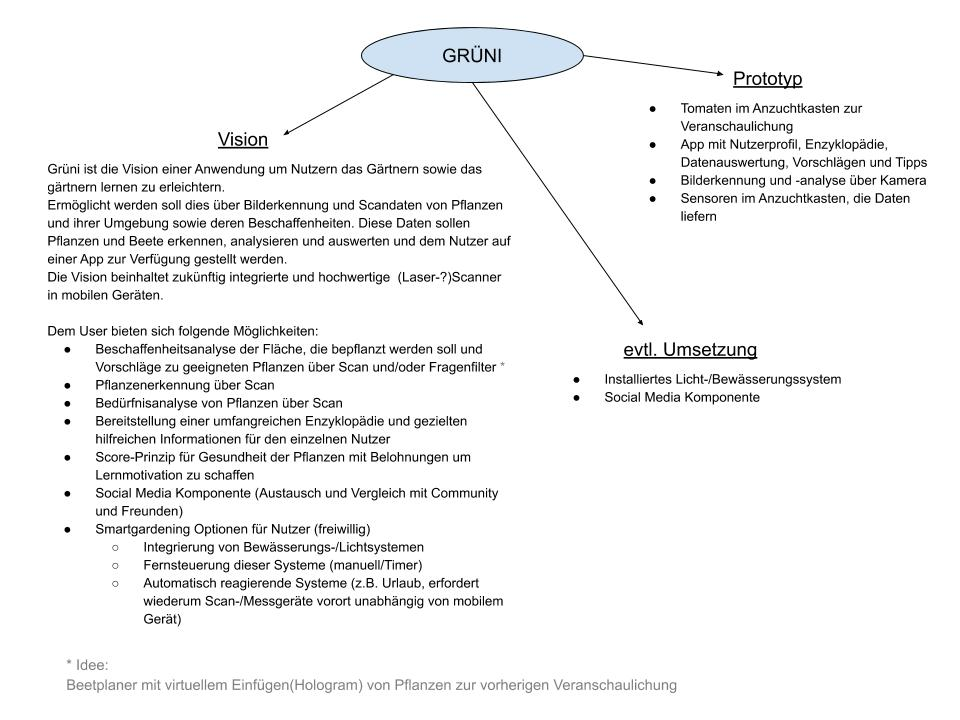
\includegraphics{img/Projektthema.jpg}
\caption{Grafik `Vision vs.~Prototyp'}
\end{figure}

Abgrenzen von der technischen \textbf{Ausstattung zur Analyse} muss man
die zur \textbf{Versorgung} der Pflanzen. Dies soll mit der Anwendung
Grüni zwar möglich sein, aber freiwillig, da weitere
Geräteinstallationen dafür nötig sind und der Lern- und
Informations-Aspekt im Vordergrund stehen sollen.

Für den Prototypen war jedoch bereits zu diesem Zeitpunkt klar, dass wir
nicht auf Sensoren verzichten werden können und auch der Wirkungsraum
spezifisch eingegrenzt sein wird. Dazu allerdings erst später mehr.

\hypertarget{aufgetretene-schwierigkeiten-und-deren-luxf6sungen}{%
\subsection{Aufgetretene Schwierigkeiten und deren
Lösungen}\label{aufgetretene-schwierigkeiten-und-deren-luxf6sungen}}

\begin{itemize}
\tightlist
\item
  Masse an Recherche-Material aussortieren und für das Projekt
  wesentliche Aspekte herausfiltern
\item
  Anforderungen an das Projekt definieren bei großer Auswahl an
  Möglichkeiten der Umsetzung
\item
  Die Innovation nicht aus dem Auge verlieren, klar definieren was
  ``anders'' ist an Grüni
\end{itemize}


\appendix

\end{document}
